\documentclass[11pt,twoside,a4paper]{article}
\usepackage[english]{babel} 
\usepackage{hyperref}
\usepackage[margin=4cm]{geometry}
\usepackage[style=apa,hyperref,doi,url,backend=biber]{biblatex}
\usepackage{csquotes}
\usepackage{graphicx}
\DeclareLanguageMapping{english}{english-apa}
\usepackage[export]{adjustbox}

\title{Emergent Architecture Design} 
\author{
	Paul Bakker, pbakker3, 4326091 \\
    Robin Borst, robinborst, 4291972 \\
    Matthijs de Groot, mawdegroot, 4171683 \\
    Julian Hols, jthols, 4247930\\
    Jan van Rosmalen, javanrosmalen, 4318609\\
}
\addbibresource{references.bib}

\begin{document}
\maketitle
\newpage
\tableofcontents
\newpage

\section{Introduction}

To implement our product we will have different design goals so we can satisfy the needs of the customer. These are described here below. In section 2 we will describe the software architecture views of our product.

\subsection{Design Goals}
\subsubsection{Usability}
The most important design goal that we have is usability. It is important that the user can execute the program really efficiently and in a rapid order. That is the reason that we made a user interface where the user can quickly select, input files, output directory and a scripting file. This allows the user to quickly change the input data and execute the on the same script and output directory.  Because the interface is intuitive, but not in the form of a wizard with dialogs, we think this is the best implementation to execute the program. This enhances the usability for the analyst as he can process a lot of data really quickly.
\subsubsection{Modularity}
The modularity design goal means that we will define the individual components well, which leads to better maintenance. Also because we work with five people it is beneficial to have good modularity as we can each work on an individual component. And good modularity also helps us greatly in realizing our next design goal.
\subsubsection{Re-usability}
The re-usability design goal means that we will be able to reuse almost all of the code for other customers. We could for example reuse most of the code to easily get the same functionality for other self-monitoring projects.
\subsubsection{Compatibility}
The compatibility design goal means that the software is able to operate with different file formats outputted by other software products. We will use this to accept multiple file formats for the import and export. The exported files then can be used by different statistics analysis programs.
\newpage
\section{Software Architecture Views}

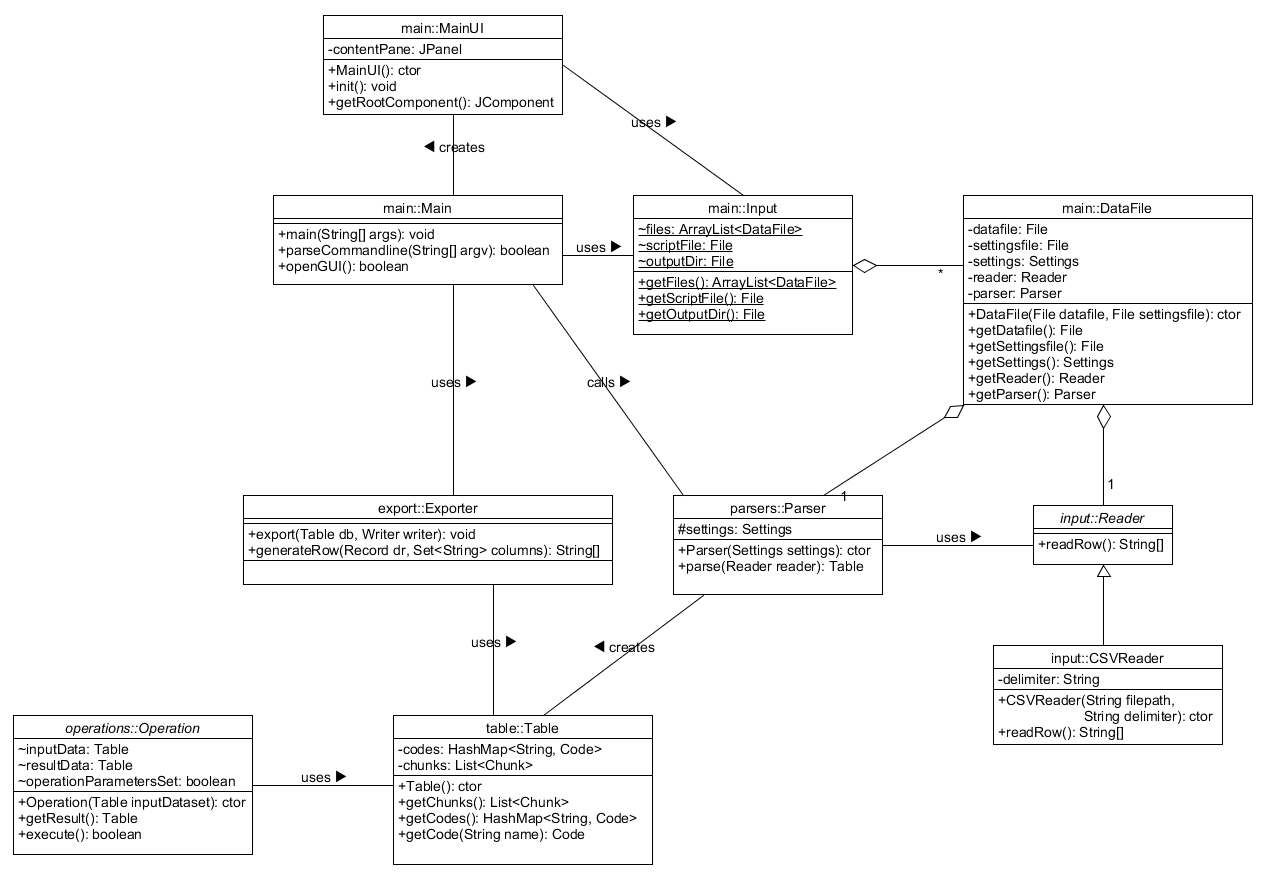
\includegraphics[scale=0.7, center]{Class_diagram.PNG}

\subsection{System derivation}
In this section we will explain how we derived our current architecture, by listing the program features.

\begin{itemize}

\item Selecting input files:\\
First of all, the input files must be selected. If no command line is used, a GUI must be shown. For this purpose we use the MainUI class to create and show a user interface.

\item Specifying input files:\\
For all input files the user must specify how the file is constructed. For this we use XML files, which can be read by our XMLReader. This reader will output a Settings object, which represents the just read XML file.

\item Reading input files:\\
For reading an input file, we implemented an abstract class Reader. This class has an abstract method readRow(), so all subclasses must specify how a row is read. So different kinds of files can be read, only a new Reader must be implemented for how to read a row.\\ 
For choosing the correct reader for a file, we have the class DataFile. This class contains all information about a file, so it can choose the correct reader.

\item Parsing input files:\\
For parsing the input files, we implemented the class Parser. This class reads a row from a file using the corresponding Reader and checks the values. To know what type the values must have, we have the Settings object. In the Settings all column types are specified. If, for example, a number is expected, but a String value is found, an exception will be thrown.

\item Representing data:\\
In the program all data must be represented. For this we use a Table, which is basically a list of Records. A Record then is basically a HashMap which maps column names to actual Values. Value is an abstract class, from which the subclass objects are generated by the Parser. These subclasses are for example NumberValue and DateValue, so we can easily know which types the values have.

\item Doing operations:\\
For doing operations on the data, we implemented an abstract class Operation. All operations can extend this class, so they have to implement an execute method. This way we use the command design pattern.

\item Specifying operations:\\
TODO: Script

\item Writing output:\\
For writing the data to a CSV file, we have the class Exporter. This class takes the Table object and output directory, which is a Writer, and writes the output to an output CSV file. 

\end{itemize}

\subsection{Subsystem decomposition}
We will divide our product into different components, which we will describe below. 

\begin{itemize}
\item The Main class:\\
The Main class contains the main method which is the first method that will be called when the user runs the program. Main will parse the command line arguments. The user can pass arguments to the program using a command line or a script. Main will also start the graphical user interface (gui) and receive the data the user inputs in the gui. After the user has input all the required data, the main method will execute the script file supplied by the user.

\item MainUI class:\\
The MainUI class contains all the code for the graphical user interface (gui). It allows the user to specify the input files in a more user friendly way than the command line. The gui asks the user to specify the script file, an output directory and a list of data files and the corresponding settings file for the data file. The Main class will initialize the mainUI and will also read the input data when the user is finished.

\item DataFile class:\\
The DataFile class provides an easy way of storing information about the data file and it's corresponding settings file. The dataFile will create  the correct Reader and Parser for the file and will read the settings file using XMLReader.

\item Settings class:\\
The Settings class is created by the XMLReader. It contains information on how to parse the file and specifies the column names and data types for each column. It is mainly used by the Parser class.

\item XMLReader class:\\
The XMLReader will be used by DataFile class to read a settings file in xml format. It outputs a Settings object.

\item Reader abstract class:\\
The reader will read the data file and provides an easy way for the Parser to read the data file. The reader allows us to add support for different file formats such as csv and xls without having to write a different Parser for each file format.

\item Parser class:\\
The parser will read data row by row from the Reader interface. For each file it parses it receives a Settings object containing information on how to parse this file. The settings object specifies the column names and the Value type of the data the column holds. The parser will create the correct Value object and add it to a Record. The parse class will output all Records after parsing into a Table data structure.

\item Value abstract class:\\
The Value abstract class allows us to easily add data types such as NumberValue, DateValue and StringValue.
The Parser will create the correct Value object that is specified for each column in the settings file.

\item Table class:\\ 
The Table class holds a table of Record objects. A record object stores a row of data in a HashMap. This way data and columns are easily added or removed from the record. The table class is created by the Parser. It is used as an input in data processing commands such as filtering and chunking. The data processes will output an updated table. Also there are fields for quick lookups. Currently there is a collection of all the chunks and of all codes.

%\item ScriptInterpreter class:\\ 
%The ScriptInterpreter class will read the script file and execute all the corresponding sequential data operations. It will output a data-structure predefined by us.

\item Exporter class:\\
The Exporter class will generate a text/csv file from a Table object. The user will be able to select the delimiter to use to separate items. For the actual writing we make use of OpenCSV's CSVWriter. We use this component because it uses Java's own classes to write lines to the output file. For the constructor we use Java's Writer and for writing a line we use a String array. 

An alternative for writing csv files is Commons CSV. We don't use this library, because it uses its own class CSVFormat. So, we found that the OpenCSV library was easier to use.

\item Operation abstract class:\\
The Operation abstract class allows us to easily add new operations to execute on the data. Each operation takes an input table and creates a result table. To create this table, the operation needs parameters to know how to perform the operation. In the next section we will explain how each operation is implemented.

\end{itemize}

\subsection{Operation implementations}

\begin{itemize}

\item Chunking (ChunkingOperation):\\
For the operation chunk we make use of the abstract class ChunkCondition. This class specifies which condition should hold for two records to be put in the same chunk. The chunks are made by iterating through the table and check whether the condition holds. If so, put the record in the current chunk, otherwise create a new chunk.\\
A list of the created chunks is saved and added to the result Table. This way the original Table can be easily iterated over, as well as over the chunks.

\item Constraints (FilterOperation):\\
For the operation constraint we use an enum containing the constraints to check between two values. For numbers for example you can get the numbers greater than or equal to a certain value. Since all Values implement Comparable, all constraints can be applied to all value types.

\item Coding (CodingOperation):\\
For the operation coding we use the design pattern Decorator. This is because coding is used among other things to recognize behavior patterns, which means recognizing sequences of events. To implement this we have an abstract class Pattern, which has an attribute nextPattern and a method findPattern. This makes it easy for us to add new Patterns.\\
The CodingOperation only has to know the first Pattern to find. When executing, the class calls findPattern on his attribute Pattern. If the called Pattern is indeed found, it calls findPattern on his successor, nextPattern. This way multiple Patterns can be combined just by defining the sequence. Because there must always be a nextPattern, we introduced a NullPattern, which defines the end of a sequence.\\ 
When a pattern is found, all records that together form the pattern are added to a Code object. This is a class containing the code name and a set of Tables (list of Records). So the frequency of a code can be easily retrieved, by retrieving the size of the set.

\item Connect (ConnectionOperation):\\
For the connection operation we merge two Table objects. Since each Record in the Table is a HashMap, new columns can be easily added to the result table. Because of the use of the HashMap, the order of the columns does not matter and columns with the same name will be merged automatically.

\item Compare (BetweenOperation and LSAOperation):\\
For comparing the time between two type of events, the BetweenOperation can calculate for each event A, how much seconds it takes for a following event B occurs. To do a Lag Sequential Analysis (lsa), the LSAOperation can be used. Contrary to other Operations, this does not return an adapted version of the inputTable, but a new table containing the LSA between event A and B.

\end{itemize}

\newpage
\subsection{Remaining UML diagrams}
Table:\\
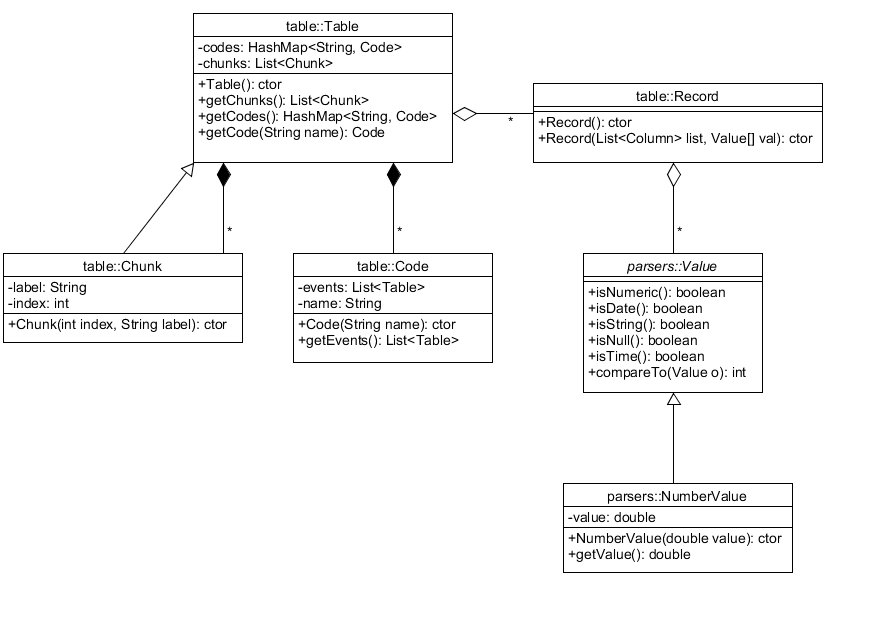
\includegraphics[scale=0.8, center]{Table_diagram.PNG}

Parser:\\
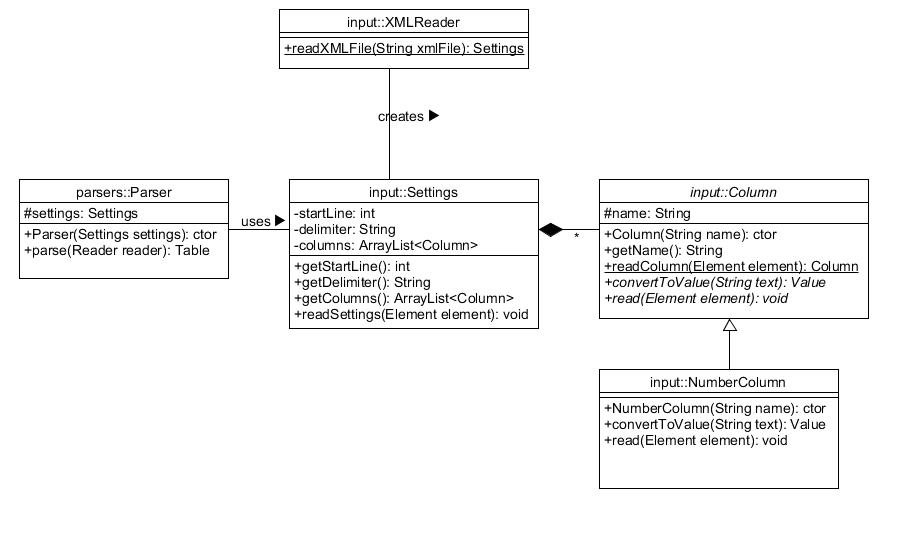
\includegraphics[scale=0.8, center]{Parser_diagram.PNG}

Operations:\\
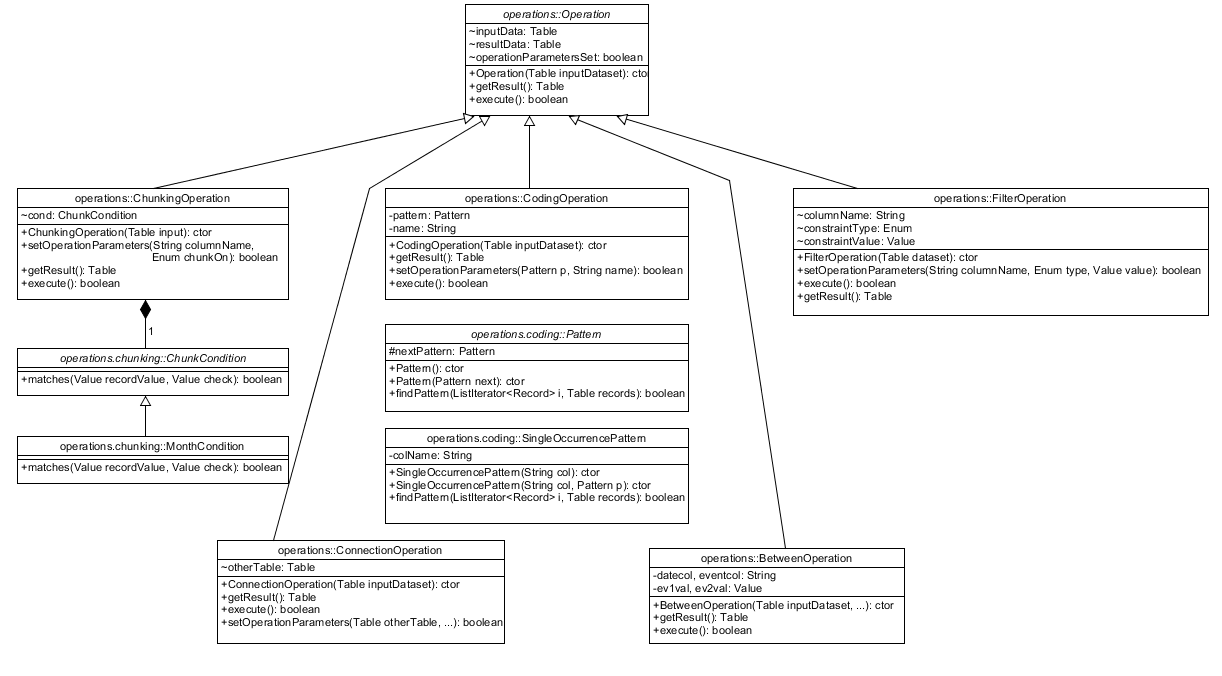
\includegraphics[scale=0.8, center]{Operations_diagram.PNG}

\end{document}